\chapter{Обзор методов построения моделей окружающего пространства БТС на основе комплексирования данных разной природы}\label{ch:ch1}

\section{Современное состояние беспилотных транспортных средств}\label{sec:ch1/sec1}

Развитие беспилотных транспортных средств является одним из наиболее активных направлений интеллектуальных роботизированных систем. Разрабатываемые решения в этой области значительно отличаются по функционалу, а также условиям, в которых они применяются. Для классификации автономного транспорта Обществом автомобильных инженеров (англ. Society of Automotive Engineers, SAE) в 2014 году были предложены шесть уровней автоматизации (SAE J3016)~\cite{sae2014taxonomy}. 

\begin{enumerate}
	\item \textbf{Уровень 0. Отсутствие автоматизации (No Automation)}
	
	
	На данном уровне водитель полностью контролирует движение транспортного средства. Рулевое управление, ускорение/торможение и выполнение манёвров осуществляются исключительно водителем. Автоматические системы, доступные на транспортных средствах данного уровня, осуществляют только информационные функции либо краткосрочно берут на себя вспомогательные функции управления транспортным средством. Примерами систем такого уровня являются системы предупреждения о сходе с полосы, СПСП (Lane Departure Warning, LDW)~\cite{chen2020lane}, системы обнаружения объектов в слепых зонах транспортного средства (Blind Spot Monitoring, BSM)~\cite{forkenbrock2014blind}, системы автоматического экстренного торможения, САЭТ (Autonomous Emergency Braking, AEB)~\cite{hulshof2013autonomous} и др.
	
	\item \textbf{Уровень 1. Вспомогательные системы (Driver Assistance)}
	
	Автоматические системы автомобиля на данном уровне могут выполнять одну из основных функций управления транспортным средством в определённых условиях, например ускорение или торможение или рулевое управление. При этом ответственность за безопасность остаётся на водителе, который обязан контролировать окружающую ситуацию и быть готовым взять управление транспортным средством на себя. Типичные примеры систем этого уровня -- адаптивный круиз-контроль (Adaptive Cruise Control, ACC)~\cite{pananurak2009adaptive} -- система, позволяющая поддерживать фиксированные скорость и дистанцию позади идущего впереди транспортного средства, а также система удержания полосы движения, СУПД (Lane Keeping System, LKS)~\cite{amditis2010situation}.
	
	\item \textbf{Уровень 2. Частичная автоматизация (Partial Automation)}
	
	На данном уровне системы транспортного средства способны одновременно выполнять и рулевое управление, и торможение/ускорение. Однако, как и на предшествующих уровнях, водитель несёт полную ответственность за безопасность движения транспортного средства. К системам данного уровня относят системы удержания полосы, которые, в отличие от аналогичных систем первого уровня, контролируют не только рулевое управление, но и способны корректировать скорость транспортного средства. Также к этому уровню принадлежат системы автоматической парковки (Automatic Parking)~\cite{ma2017research}.
	
	\item \textbf{Уровень 3. Условная автоматизация (Conditional Automation)}
	
	Автоматические системы автомобиля на этом уровне способны полностью осуществлять управление транспортным средством без участия водителя в ограниченных условиях: как правило, это определённый тип дороги (автомагистрали с отчётливо распознаваемой разметкой) и хорошие погодные условия. В случае возникновения нестандартной ситуации на дороге система должна своевременно передать управление транспортным средством водителю. Соответственно, в отличие от предшествующих уровней, от водителя не требуется постоянное слежение за окружающей обстановкой, но он должен быть готов к управлению транспортным средством в нештатных ситуациях. Пример такой системы -- ассистент движения в пробках (Traffic Jam Assist)~\cite{rao2019test}.
	
	\item \textbf{Уровень 4. Высокая автоматизация (High Automation)}
	
	Аналогично предыдущему уровню, системы автомобиля уровня 4 способны осуществлять полное управление транспортным средством в чётко определённых сценариях. От систем 3-го уровня их отличает способность самостоятельного завершения поездки или возвращения в безопасное состояние в случае возникновения внештатной ситуации и отсутствия реакции от водителя. Как следствие, на автомобили данного уровня не накладывается требование к обязательному наличию водителя. К системам этого уровня относят беспилотное такси и автоматизированные грузовые транспортные средства.
	
	\item \textbf{Уровень 5. Полная автоматизация (Full Automation)}
	
	На данном уровне автономности системы автомобиля способны осуществлять полное управление транспортным средством без ограничения на условия эксплуатации. Автомобили данного уровня не требуют наличия механизмов ручного управления, таких как педали торможения/ускорения, рулевое колесо и пр. На сегодняшний день не существует транспортных средств, обладающих 5-м уровнем автоматизации, несмотря на большое количество работ, направленных на их создание.
	
\end{enumerate}

В настоящее время идёт бурное развитие технологий, направленных на усовершенствование беспилотных транспортных средств, обладающих 4-м уровнем автоматизации, а также создание транспортных средств с 5-м уровнем автоматизации. Среди проектов по разработке таких транспортных средств можно выделить Waymo~\cite{schwall2020waymo}, Tesla~\cite{ingle2016tesla}, Яндекс~\cite{Хабр2021}, Baidu Apollo~\cite{fan2018baidu} и др. Несмотря на то, что данные проекты показывают высокую степень автономности~\cite{freedman2018autonomous}, перед отраслью стоит множество задач, требующих решения для повышения уровня безопасности движения беспилотных транспортных средств, что будет способствовать внедрению данных технологий в повседневное использование~\cite{khan2022level}. Одна из таких задач -- разработка надёжных систем восприятия транспортного средства, отвечающих за построение точной и полной модели окружающего пространства. В рамках данной работы исследуются и предлагаются алгоритмы построения таких моделей.

\section{Модели окружающего пространства БТС}\label{sec:ch1/sec2}

В робототехнике под моделью окружающего пространства понимается приближённое описание окружающих БТС объектов: их наличие и положение в некоторой окрестности транспортного средства. Помимо информации о положении объектов, такая модель может описывать их скорость и предполагаемую траекторию движения. Также модель может описывать форму и расположение проезжей части, слепых зон транспортного средства (как вызванных окклюзией, так и обусловленных отсутствием показаний датчиков для соответствующей области пространства), а также объектов транспортной инфраструктуры: полос разметки, дорожных знаков, бордюров, светофоров и т.д. 

В рамках данной работы исследуются двумерные модели -- модели, проецирующие объекты, окружающие БТС, на плоскость его движения. Такие модели не хранят информацию о высоте объекта и его положении над землёй, т.к., как правило, эти данные избыточны для решения задачи планирования движения колёсного транспорта. В то же время следует отметить, что среди предложенных на сегодняшний день моделей существуют и трёхмерные~\cite{yudin2025}. Так, в работе~\cite{oliveira2015scene} окружающая сцена представлена совокупностью полигонов, в работе~\cite{dryanovski2010multi} пространство разбивается трёхмерной сеткой, каждому элементу которой сопоставляется вероятность нахождения в нём препятствия, а в работе~\cite{feng2025survey} в отдельный класс выделены модели, описывающие окружающее пространство как облако точек. 

Среди существующих двумерных моделей можно выделить три категории:

\begin{enumerate}
	\item \textbf{Объектно-ориентированные представления}. В них окружающая сцена описывается как множество объектов. Как правило, объект представлен в виде ограничивающего параллелепипеда: положением его центра, ориентацией и габаритами~\cite{mao20233d}. Дополнительно описание объекта может содержать тип (транспортное средство, пешеход, животное и т.д.), а также линейные и угловые скорость и ускорение~\cite{caesar2020nuscenes, pieroni2024, wang2024}, предсказываемую траекторию перемещения~\cite{altche2017lstm}. Такие модели имеют достаточно краткую форму записи: множество векторов, описывающих отдельный объект, что делает их вычислительно эффективными. В то же время они ограничены в возможности описания объектов сложной формы: тягачи с полуприцепами, перевёрнутые машины, объекты нетипичной формы.
	
	\item \textbf{Сеточные представления}. Модели этой категории призваны обойти ограничение предыдущей категории и описывать объекты с произвольной геометрией. В них пространство вокруг транспортного средства разбивается на сетку фиксированного разрешения, каждая клетка которой хранит информацию о наличии (или вероятности наличия) препятствия в соответствующей области~\cite{thrun2003learning}. Такое представление получило название карты проходимости пространства~(Occupancy Grid Map, OGM). К этой же категории относятся динамические карты проходимости пространства~(Dynamic Occupancy Grid Map, DOGMa)~\cite{dryanovski2010multi}, в них для клеток, в которых обнаружено препятствие, добавляется информация о его скорости и направлении движения. Модели этой категории также чаще, чем объектно-ориентированные модели, учитывают неклассифицируемые объекты: мусор, открытые люки, бордюры и т.п., что делает их более надёжным представлением окружающей сцены. Однако более детальное описание сцены приводит к большему размеру структуры данных в памяти компьютера, что негативно влияет на вычислительную сложность алгоритмов, работающих с моделями в этой категории. Ограниченная разрешающая способность данных моделей также может рассматриваться как недостаток для некоторых задач автономной навигации.
	
	\item \textbf{Непрерывные представления}. Как и модели прошлой категории, модели непрерывного представления стремятся описывать объекты со сложной геометрией. Однако в отличие от сеточных представлений модели этой категории представляют пространство как непрерывное отображение $\mathbb{R}^2 \rightarrow O$, где каждой точке плоскости движения транспортного средства сопоставляется некоторая характеристика: бинарная классификация принадлежности точки проезжей части дороги ($O=\{0,1\}$), класс объекта ($O=\{0,\dots N\}$), плотность вероятности нахождения препятствия в данной точке ($O=\mathbb{R}^+$) и т.п. Таким образом, модели данной категории имеют бесконечную степень детализации, что позволяет обойти главное ограничение сеточных представлений. Недостаток же моделей данной категории заключается в том, что алгоритмы для их построения и обновления сложнее в реализации, а вычислительная сложность может быть хуже, чем у предыдущих двух категорий (для сеточных представлений последнее зависит от требований к размеру и разрешению сетки). Примерами таких представлений служат полигональные раскраски (Polygonal Random Field, PRF)~\cite{paskin2012robotic}, мультимодальное нормальное распределение~\cite{yuan2023generating}.
\end{enumerate}

В рамках данной диссертационной работы будут предложены алгоритмы для построения и обновления карты проходимости пространства из категории сеточных представлений. Данный выбор основан на широком распространении модели, вычислительной простоте и, как будет показано в работе, масштабируемости относительно числа датчиков, участвующих в обновлении модели. Опишем подробнее эту модель и методы её построения.

Представление окружающего пространства в виде карты проходимости пространства было впервые предложено в работах Альберто Элфеса и Ханса Моравека~\cite{elfes1989occupancy, Moravec_1988}. В рамках данного представления окружающее пространство разбивается на двумерную сетку $M$, каждой клетке которой $m_i$ сопоставляется вероятность нахождения препятствия в пространстве $p(m_i)$, ограниченном этой клеткой. В работе~\cite{moravec1985high} те же авторы расширили модель карты проходимости пространства, включив в неё обратную модель наблюдения -- вероятностную модель, моде­лирующую процесс измерений датчика и учитывающая принцип работы, а также особенности среды, в которой производятся наблюдения. Расширение модели позволило сформулировать алгоритм уточнения карты проходимости пространства на основании показаний датчика. В рамках данной модели дополнительно делается предположение, что каждая вероятность занятости клетки в карте проходимости не зависит от вероятностей занятости других клеток карты. Для каждой клетки вычисляется величина так называемого логарифма шансов:

% На сегодняшний день предложено множество алгоритмов построения карты проходимости пространства. Их реализация сравнительно проста в случае, если информация об окружающем пространстве поступает от единственного датчика. Примеры таких систем представлены в статьях~\autocite{wang2018single} и \autocite{luo2019probability}. Однако для большинства практических задач единственного датчика недостаточно из-за ограниченного поля зрения, невозможности полностью компенсировать зашумлённость входных данных и общих ограничений, обусловленных принципом его работы.  Так, например, использование камер видимого диапазона невозможно в ночное время суток, а качество работы лидаров снижается в условиях сильных осадков.    

%В данной работе будет реализован алгоритм построения карты проходимости пространства   мы предлагаем модификацию алгоритма, относящегося к первой группе -- картирование на основе Байесовского вывода с использованием обратной модели наблюдения. Выбор данного подхода обусловлен простотой модификации базовой реализации, низкой вычислительной сложностью, а также хорошей масштабируемостью при увеличении количества используемых источников входных данных.  Первая версия данного алгоритма была представлена в работе Моравица~\autocite{Moravec_1988}. 

\begin{equation}
	l_{t,i} = \ln\dfrac{p(m_i|z_{1:t}, x_{1:t})}{1 - p(m_i|z_{1:t}, x_{1:t})},
\end{equation}
где $p(m_i|z_t, x_t)$ -- вероятность занятости $i$-й клетки карты, при условии, что к моменту времени $t$ БТС прошёл траекторию $x_{1:t}$, и его датчики давали показания $z_{1:t}$. Заметим, что здесь используется обратная причинно-следственная зависимость: измеряется вероятность причины (занятость пространства), при условии наступления его следствия (показания датчика), чем и обусловлено название модели. С получением новых данных значения в тех клетках, о которых появились новые данные (иными словами, которые попали в область видимости датчика), обновляются по следующей формуле:

\begin{equation}
	l_{t,i} = l_{t-1,i} + \ln\dfrac{p(m_i|z_t, x_t)}{1 - p(m_i|z_t, x_t)} - l_{0,i},
	\label{eq:log_odd_upd}
\end{equation}
где $l_{0,i} = \ln\dfrac{p(m_i)}{1 - p(m_i)}$ -- логарифм шансов, посчитанный для априорной вероятности занятости клетки. Зачастую о карте проходимости не делается априорных предположений и $p(m_i)$ устанавливают равным $0,5$, что приводит к $l_{0,i} = 0$. 

Такой формат обновления удобен, так как позволяет независимо друг от друга посчитать значение $\ln\dfrac{p(m_i|z_t, x_t)}{1 - p(m_i|z_t, x_t)} - l_{0,i}$, на основании полученных данных от каждого датчика, а затем просто добавить полученное значение к уже имеющейся карте проходимости (при условии атомарности данной операции). 


\section{Обзор используемых в колёсной робототехнике датчиков и их ограничения}\label{sec:ch1/sec3}

Обновление любой модели окружающей сцены производится на основании показаний датчиков, установленных на БТС. Основные датчики, применяемые в колёсной робототехнике для построения модели, -- лидары, радары, сонары и камеры~\cite{vargas2021overview}.

\begin{enumerate}
	
\item \textbf{Радары (Radio Detection and Ranging, RADAR)}. Технология, основанная на создании радиоволн и регистрации их отражений от объектов. По времени регистрации и степени затухания отражённой волны датчик определяет расстояние до объекта и его скорость. Радары разделяют на радары дальнего диапазона (РДД) и короткого диапазона (РКД)~\cite{сысоева2007актуальные}. Первые обладают наибольшей дальностью видимости (около 250~м) среди упомянутых датчиков и используются для обнаружения препятствий на пути движения машины. Вторые обладают меньшей дальностью, но лучшим разрешением и могут быть использованы для реализации систем парковки и перестроения между полосами движения. В то же время радары обладают низким угловым разрешением и могут давать ложные срабатывания из-за металлических конструкций, например, решёток ливневых канализаций в поле видимости, и переотражений сигнала излучателя. 
	
\item \textbf{Лидары (Light Detection and Ranging, LiDAR)}. Технология, начавшая развитие во второй половине XX века, в 1960-х годах, в космической и авиастроительной сферах~\cite{wandinger2005introduction}. Принцип работы схож с радаром, но вместо радиоволн использует пучки инфракрасного спектра. Существует два типа лидаров: механические и твердотельные. В механическом лидаре источники и приёмники сигнала вращаются на высокой (от 600 оборотов в минуту) скорости. В твердотельном лидаре источник и приёмник остаются неподвижны, а изменение направления сканирующего луча производится путём вращения призмы или зеркала, через которые он проходит. Помимо измерения расстояния до объекта лидары способны регистрировать его светоотражательную способность, что может быть применено, например, для детекции разметки. Лидары обладают высокой точностью и лучшим разрешением, чем радары, и хорошей дальностью обзора. Однако, как и радары, лидары требовательны к погодным условиям: качество измерений снижается в условиях тумана и/или осадков. Также ограничивающим фактором для использования лидаров является их дороговизна, из-за этого многие компании, занимающиеся разработкой беспилотных автомобилей, вынуждены отказываться от лидаров в пользу альтернативных способов детекции местонахождения машины и построения маршрута движения. Лидары могут использоваться для распознавания и классификации объектов, создания трёхмерных карт.	

\item \textbf{Камеры}. Наиболее распространённые датчики~\cite{ignatious2022overview}, используемые в колёсной робототехнике. В отличие от остальных описанных датчиков, камеры -- пассивные датчики: они не излучают никаких сигналов. Для активных же датчиков отдельной проблемой является взаимная интерференция. Это позволяет без опасений использовать большое количество камер без необходимости синхронизировать их работу друг с другом. В основном в БТС используют камеры видимого (400--780~нм) спектра, но также встречаются модели, использующие камеры инфракрасного спектра. Камеры обладают наилучшим разрешением среди описанных датчиков, но не способны измерять расстояние до объектов. Использование нескольких камер в связке позволяет использовать алгоритмы стереозрения для измерения расстояния, однако точность и дальность этих измерений ниже, чем у лидаров и радаров. Камеры используются для захвата изображений, которые затем обрабатываются с помощью алгоритмов компьютерного зрения. Камеры в компьютерном зрении широко используются в различных областях, таких как робототехника, автоматическое управление производственными процессами, медицинская диагностика, безопасность, распознавание лиц, автоматическое управление транспортом, анализ изображений и многих других. 

\item \textbf{Сонары}. Как лидары и радары, принцип работы сонаров основан на измерении времени регистрации отражения волн от объектов, однако в сонарах используются ультразвуковые (40--70~кГц) волны~\cite{kleeman2016sonar}. Данные волны не слышны и не могут нанести вред слуху человека, что немаловажно, поскольку громкость создаваемого импульса достигает 100~дБ. Сонары обладают наименьшей областью обзора (менее десятка метров) и потому, как правило, используются для систем парковки. Сонары используются для измерения расстояния до объектов и создания трёхмерной модели окружающей среды. Они работают на основе эхолокации, отправляя звуковые импульсы и затем регистрируя отражённые от объектов сигналы. Полученные данные могут быть обработаны компьютером для определения расстояния и формы объектов. Одним из наиболее распространённых применений сонаров является их использование при парковке БТС. Также сонары могут использоваться в системах обнаружения движущихся объектов, таких как пешеходов и других транспортных средств.
\end{enumerate}

Из описания датчиков следует, что каждый тип датчика обладает рядом преимуществ и недостатков. Использование нескольких датчиков разных типов на одном транспортном средстве позволяет компенсировать недостатки отдельных датчиков и добиться повышения качества восприятия, тем самым повышая безопасность движения и открывая новые сценарии применения беспилотных транспортных средств. Сводное сравнение характеристик рассмотренных датчиков приведено в таблице~\cref{tab:sensors}.

\begin{table}[h!]
	\small
	\centering
	\begin{tabular}{|l|c|c|c|c|}
		\hline
		\textbf{Характеристика}          & \textbf{Лидар} & \textbf{Радар} & \textbf{Камера} & \textbf{Сонар}\\
		\hline
		Разрешение                       & Среднее    & Низкое  & Высокое & Низкое  \\
		Дальность области обзора         & 150~м & 250~м & 200~м & 5~м \\
		Устойчивость к погодным условиям & Средняя    & Высокая & Низкая  & Высокая \\
		Чувствительность к условиям освещения & Нет   & Нет     & Высокая & Нет     \\
		Информация о дистанции           & Да         & Да      & Нет     & Да      \\
		Вычислительная нагрузка обработки& Средняя    & Низкая  & Высокая & Низкая  \\
	    Стоимость                        & Высокая    & Средняя & Низкая  & Низкая  \\
		\hline
	\end{tabular}
	\caption{Сравнение характеристик датчиков, используемых в колёсной робототехнике}\label{tab:sensors}
\end{table}


\section{Методы комплексирования данных}\label{sec:ch1/sec4}

На сегодняшний день предложено множество алгоритмов построения карты проходимости пространства. Их реализация сравнительно проста в случае, если информация об окружающем пространстве поступает от единственного датчика. Примеры таких систем представлены в статьях~\autocite{wang2018single} и \autocite{luo2019probability}. Однако для большинства практических задач единственного датчика недостаточно из-за ограниченного поля зрения, невозможности полностью компенсировать зашумлённость входных данных и общих ограничений, обусловленных принципом его работы.

Чтобы получить более точную модель окружения и повысить безопасность движения БТС, на них устанавливают несколько датчиков. Примеры систем с несколькими датчиками описаны в работах~\autocite{xu2020data, rosenband2017inside}. Встречаются как системы, использующие несколько датчиков одного типа (например, камеры, как в работах~\autocite{bertozzi1998experience, bochare2025cameraonlybirdseyeview}), так и комбинирующие различные датчики, например: 
\begin{itemize}
	\item лидары и радары. Примеры таких БТС представлены в~\autocite{gohring2011radar, wang2023bi, song2024lirafusion};
	\item лидары и камеры~\autocite{tibebu2021lidar, caltagirone2019lidar, liu2023real};
	\item и другие комбинации~\autocite{yao2023radar, nabati2021centerfusion, s23063335}. 
\end{itemize}

Алгоритмы построения модели окружающего БТС пространства для таких систем в общем случае генерируют модель достаточно полную и точную, но вынуждены решать задачу комплексирования данных для разрешения противоречий в показаниях разных датчиков. Существуют разные алгоритмы, осуществляющие комплексирование данных, которые можно разделить на три группы~\cite{s21062140}:

\begin{enumerate}
	\item Раннее комплексирование -- необработанные данные с датчиков объединяются в один пакет данных и передаются системе для последующего анализа. Примером такой агрегации является построение карты глубины в стереокамере, как например в работе~\cite{smagina2018obstacle}.
	
	\item Промежуточное комплексирование -- по сырым данным с датчиков вычисляются отдельные признаки (в общем случае отличные для каждого из датчиков), которые затем объединяются для дальнейшего решения задачи. Так в работах~\cite{fan2022deep, jiang2021manipulator} данные с разных датчиков обрабатываются разными нейросетевыми моделями, после чего выходные тензоры конкатенируются.
	
	\item Позднее комплексирование -- для каждого датчика целевая задача (в нашем случае построение модели окружающего БТС пространства) решается отдельно, что даёт независимую гипотезу. На основе этих гипотез более высокоуровневый алгоритм вычисляет итоговое решение.
\end{enumerate}


Для существующих алгоритмов комплексирования данных в контексте задачи построения карты проходимости пространства в работе \autocite{sasiadek2002sensor} представлена классификация по трём группам:

\begin{enumerate}
	\item Методы, использующие вероятностные модели. К ним относятся байесовский вывод, теория Демпстера"--~Шафера, робастные методы и т.д.
	\item Методы, использующие метод наименьших квадратов (МНК): фильтр Калмана, методы оптимизации, эллипсоиды неопределённости (англ. uncertainty ellipsoids) и пр.
	\item Методы интеллектуального комплексирования: методы нечёткой логики, нейросетевые и генетические алгоритмы. 
\end{enumerate}

В настоящее время продолжается активная разработка алгоритмов каждой из трёх групп. Примером актуальных исследований в первой группе является работа~\autocite{duong2022autonomous}, в которой используется метод релевантных векторов (метод машинного обучения, использующий байесовский вывод) для построения непрерывной карты проходимости пространства. Во второй группе можно выделить работу~\autocite{9274841}, в которой положение динамических препятствий на карте обновляется с помощью фильтра Калмана. Стоит отметить, что в данной работе обновление информации о статических препятствиях происходит с помощью байесовского вывода, поэтому предлагаемый алгоритм является объединением методов из двух представленных групп. Наконец, не менее активно развиваются алгоритмы третьей группы, одним из которых является модель глубокого обучения BEVFusion, представленная в работе~\autocite{liu2024bevfusionmultitaskmultisensorfusion}.

\section{Алгоритмы проецирования данных камеры на плоскость движения БТС}\label{sec:ch1/projection}

Как отмечено в разделе~\cref{sec:ch1/sec3}, камера является наиболее распространённым датчиком в колёсной робототехнике, однако она не позволяет непосредственно измерить расстояние до наблюдаемых объектов. Результаты обработки изображения, например, визуальные детекции объектов и семантическая сегментация, получаются в однородной системе координат изображения, тогда как двумерные модели окружающего пространства, рассмотренные в разделе~\cref{sec:ch1/sec2}, описывают плоскость движения в трёхмерной системе координат БТС. Поэтому учёт визуальных данных в таких моделях требует отдельного алгоритма проецирования, от точности которого напрямую зависит корректность положения препятствий в итоговой модели.

Изображение задаёт лишь направление на наблюдаемый объект, поэтому для восстановления расстояния до него требуется либо дополнительное предположение о геометрии сцены, либо дополнительный источник данных. Определяющим для точности проецирования является то, какая модель поверхности движения БТС при этом используется, и по этому признаку существующие подходы разделим на три группы: 

\begin{enumerate}
    \item \textbf{Проецирование с использованием геометрических предположений о поверхности движения.} Если внутренняя и внешняя калибровки камеры известны, а поверхность движения считается плоскостью, то соответствие между плоскостью изображения и плоскостью движения задаётся проективным преобразование. Уравнение данной плоскости может быть фиксированным, либо пересчитываться на данных, регистрируемых датчиками, например, широкое применение получил способ поиска плоскости в облаке точек с лидаров с помощью метода RANSAC~\cite{fischler1981}. Проективное преобразование применяется как для проецирования всего изображения на вид сверху, так и для проецирования отдельных признаков: нижних границ детекций, разметки, границ проезжей части. Пример системы, использующей данный тип проекции, -- система GOLD~\cite{bertozzi1998experience}. Достоинствами методов этой группы являются вычислительная простота и отсутствие необходимости в обучении; кроме того, при использовании единственной камеры иного источника информации о геометрии сцены попросту нет. Основной их недостаток -- само предположение о плоскости поверхности движения. Оно нарушается как из-за рельефа местности, так и в силу требований к конструкции дорожного покрытия: согласно СП~34.13330.2012~\cite{sp34_2012} покрытие имеет двускатный поперечный профиль на прямых участках и односкатный на виражах. Дополнительным источником погрешности является отклонение фактической внешней калибровки от измеренной, вызванное загрузкой БТС, работой подвески и смещением датчиков при длительной эксплуатации БТС. Ошибка проецирования при этом растёт с удалением от камеры.
    \item \textbf{Проецирование с восстановлением формы поверхности движения.} Если БТС оснащён дальномерным датчиком, предположение о плоскости можно заменить оценкой формы поверхности $z = z(x, y)$, полученной по измерениям, и выполнять проецирование уже на эту поверхность. В качестве примеров такого проецирования выступают методы, основанные на разбиении облака точек сеткой в полярных координатах с последующей аппроксимацией высоты земли в каждом секторе, предложены в работах Химмельсбаха~\cite{himmelsbach2010fast} и Зермаса~\cite{zermas2017fast}; их развитием является алгоритм Patchwork~\cite{lim2021patchwork}, использующий кусочную аппроксимацию поверхности с оценкой достоверности каждого участка. Наиболее общим является представление поверхности земли как реализации гауссовского процесса~\cite{rasmussen2003gaussian}: такой подход не требует ни плоскостной, ни кусочно-плоскостной модели и позволяет оценить дисперсию предсказания, но обладает большой вычислительной сложностью по отношению к числу точек в обучающей выборке: $O(n^3)$, где $n$ -- число точек. Это затрудняет его применение в режиме реального времени. Применение регрессии на основе гауссовских процессов к выделению точек земли рассмотрено в работе Чена~\cite{chen2014gaussian}.
    \item \textbf{Обучаемые преобразования в вид сверху.} Третью группу образуют нейросетевые методы, выполняющие преобразование признаков изображения в вид сверху без явно заданной модели поверхности: геометрия сцены восстанавливается неявно, в процессе обучения. В работе Филиона~\cite{philion2020lift} для каждого пикселя изображения предсказывается распределение по глубине, после чего признаки проецируются в трёхмерное пространство на сетку вида сверху с учётом веса предскзанного распределения. В работе Ли~\cite{li2022bevformer} преобразование реализовано с применением механизма внимания над обучаемыми запросами, соответствующими клеткам сетки. Модель BEVFusion~\cite{liu2023bevfusion, liu2024bevfusionmultitaskmultisensorfusion} объединяет в едином представлении вида сверху признаки камер и лидаров. Методы этой группы демонстрируют высокое качество, однако требуют графического ускорителя для инференса, размеченных мультимодальных наборов данных для обучения и переобучения при изменении состава и расположения датчиков БТС, что ограничивает их применимость в условиях, рассматриваемых в настоящей работе.
\end{enumerate}

Результатом проецирования любым из перечисленных способов является множество точек либо полигон на плоскости движения БТС. Потребители модели окружающего пространства, как правило, не работают с таким представлением непосредственно, и тому есть две причины. Во-первых, в измерениях датчиков присутствует только обращённая к ним часть объекта, поэтому проекция систематически занижает занимаемую объектом область: недоступная для наблюдения часть объекта не будет учтена ни в модели, ни, следовательно, при планировании пути. Во-вторых, сложившимся интерфейсом между подсистемой восприятия и последующими подсистемами БТС служит описание объекта ориентированным ограничивающим параллелепипедом либо прямоугольником: в этой форме размечены общепринятые наборы данных~\cite{caesar2020nuscenes}, в ней формулируется задача в обзорной литературе по трёхмерной детекции~\cite{mao20233d}, её же принимают на вход алгоритмы предсказания траекторий окружающих объектов~\cite{altche2017lstm} и алгоритмы планирования пути, работающие с представлением препятствий в виде фигур ненулевой площади~\cite{petrovskaya2008model}. Поэтому проецирование, как правило, дополняется этапом вписывания полученной проекции в ориентированную ограничивающую рамку.

Простейшим решением этой задачи является построение рамки минимальной площади, для которого существует алгоритм с линейной по числу вершин выпуклой оболочки вычислительной сложностью~\cite{arnon1983linear}. В работе Ванга~\cite{Wang2021} для кластеров лидарных точек предложено семейство методов, использующих главные компоненты множества точек, наибольшую диагональ и вписанный треугольник. В работе Чжана~\cite{zhang2017efficient} для той же задачи предложено вписывание в L-образную модель: точки кластера считаются принадлежащими двум смежным ортогональным сторонам объекта, а ориентация рамки определяется перебором угла с фиксированным шагом. Общим ограничением перечисленных методов является то, что они разработаны для кластеров лидарных точек, природа которых отличаются от таковых для проекции визуальной детекции; кроме того, определение ориентации рамки перебором угла требует вычислительных затрат, пропорциональных числу проверяемых ориентаций.

Таким образом, существующие подходы к проецированию данных камеры на плоскость движения БТС либо опираются на предположение о плоской поверхности движения и потому вносят растущую с расстоянием погрешность, либо требуют обучения и вычислительных ресурсов, недоступных на бортовом вычислителе при одновременной обработке данных нескольких датчиков. Методы вписывания проекции в ориентированную рамку, в свою очередь, разработаны для лидарных кластеров и не учитывают специфику проекции визуальной детекции. Разработка вычислительно эффективных алгоритмов проецирования визуальных детекций и семантической сегментации проезжей части, не использующих предположение о плоской поверхности движения, а также алгоритма вписывания полученной проекции в ориентированную ограничивающую рамку составляет содержание главы~\cref{ch:ch2}.

\section{Влияние числа источников данных на время обновления карты проходимости пространства}\label{sec:ch1/performance}

В разделах~\cref{sec:ch1/sec3} и~\cref{sec:ch1/sec4} показано, что увеличение числа и разнообразия датчиков повышает полноту и достоверность модели окружающего пространства. Однако каждый дополнительный источник данных увеличивает вычислительную нагрузку на бортовой вычислитель БТС, а следовательно, и задержку между моментом регистрации данных и моментом, когда эти данные учтены в модели. Рассмотрим, как эта задержка формируется и какие ограничения она накладывает.


Обозначим через $\Delta t$ время между регистрацией данных датчиком и завершением обновления модели. Процесс обновления можно условно разделить на четыре составляющие: передачу данных от датчика к вычислителю; извлечение из них признаков (визуальтных детекций, семантической сегментации изображения, семантической сегментации облака точек и так далее); преобразование признаков в общий для всех источников формат; добавление результатов измерения в итоговую модель. Первые три составляющие выполняются для каждого источника независимо и потому допускают параллельное вычисление. Последняя составляющая является операцией над разделяемым ресурсом -- общей картой проходимости пространства -- и потому, в общем случае, требует синхронизации потоков вычислений. Заметим, что при использовании специальных структур данных, допускающих параллельное обновление, последний шаг также может быть выполнен параллельно, однако разработка подобных структур требует усложнения алгоритмов построения модели и редко встречается среди существующих реализациях. Так, в программном комплексе navigation2~\cite{macenski2020marathon} карта представлена набором слоёв, каждый из которых соответствует отдельному источнику данных. С заданой периодичностью доступ к слоям на запись блокируется для аггрегации их в единую модель и передачу результата получателям. 

Библиотека grid\_map~\cite{fankhauser2016universal}, предоставляющая универсальное представление многослойной сетки, не содержит встроенных средств одновременного обновления карты несколькими источниками. В библиотеке OctoMap~\cite{hornung2013octomap}, реализующей трёхмерную карту занятости на основе октодерева, операция вставки измерения не является потокобезопасной, и синхронизация возлагается на использующее её приложение. Аналогичным образом организовано построение сеточных моделей в программной платформе Autoware~\cite{kato2018autoware}. Отдельное направление составляют реализации, использующие графические ускорители: в работе Хомма~\cite{homm2010efficient} на графическом ускорителе распараллелено вычисление вклада отдельного датчика по клеткам карты, в работе Нусса~\cite{nuss2018random} тем же способом реализовано построение динамической карты проходимости в реальном времени. Однако распараллеливанию в этих работах подвергается вычисление вклада одного источника, тогда как объединение вкладов разных источников по-прежнему выполняется последовательно. Неблокирующие структуры данных, позволяющие нескольким потокам исполнения одновременно изменять общий объект без использования примитивов взаимного исключения~\cite{michael1996simple, herlihy2012art, fog2014lists}, к задаче построения карты проходимости пространства, насколько известно автору, ранее не применялись.

Оценим количественно, к каким ограничениям приводит последовательное внесение данных в карту. Пусть $S$ -- число источников данных, участвующих в обновлении карты. Согласно результатам профилирования программного комплекса, приведённым в разделе~\cref{sec:ch4/perf} главы~\cref{ch:ch4}, время одного цикла обновления карты составляет $3{,}03$~мс при одном источнике данных и $22{,}78$~мс при восьми. Линейная аппроксимация по этим двум точкам даёт оценку

\begin{equation}
	\Delta t(S) \approx \Delta t_0 + \delta S, \quad \Delta t_0 \approx 0{,}2~\text{мс}, \quad \delta \approx 2{,}8~\text{мс},
	\label{eq:delay_model}
\end{equation}
где $\delta$ -- вклад одного дополнительного источника данных. Линейный характер зависимости объясняется тем, что фрагменты, сформированные разными источниками, вносятся в карту последовательно, и фрагмент, оказавшийся в очереди последним, ожидает завершения обработки всех предшествующих.

Задержка $\Delta t$ приводит к двум следствиям. Во-первых, за это время БТС, движущийся со скоростью $v$, проходит расстояние $s = v \Delta t$, на которое препятствие оказывается смещено на карте относительно своего истинного положения. При $S = 8$ и $v = 60$~км/ч это смещение составляет $0{,}38$~м, при $S = 16$ -- $0{,}76$~м, что при типичном разрешении карты $0{,}2$~м соответствует систематической ошибке в две и четыре клетки. Во-вторых, из требования, чтобы карта обновлялась не реже, чем БТС проходит одну клетку, то есть $\Delta t(S) \le \Delta x / v$, где $\Delta x$ -- размер клетки карты, следует ограничение на число источников данных, которые могут быть учтены в модели без потери её актуальности. Результаты расчёта для $\Delta x = 0{,}2$~м приведены в таблице~\cref{tab:sensors_limit}.

\begin{table}[h!]
	\centering
	\caption{Предельное число источников данных при последовательном обновлении карты проходимости пространства}\label{tab:sensors_limit}
	\begin{tabular}{|l|c|c|c|}
		\hline
		\textbf{Скорость движения БТС} & \textbf{20 км/ч} & \textbf{40 км/ч} & \textbf{60 км/ч} \\
		\hline
		Допустимая задержка обновления, мс & 36 & 18 & 12 \\
		Предельное число источников данных & 12 & 6 & 4 \\
		\hline
	\end{tabular}
\end{table}

Приведённая оценка опирается на ряд допущений: рассматривается только этап внесения фрагментов в карту, зависимость~\cref{eq:delay_model} экстраполирована по двум измерениям, а сами измерения получены на конкретной вычислительной платформе (раздел~\cref{sec:experiments}). Тем не менее порядок величин показателен: при наборе датчиков, типичном для грузового БТС, этап внесения данных в карту становится ограничивающим фактором уже на скоростях, характерных для движения по дорогам общего пользования. Следовательно, для масштабирования модели окружающего пространства по числу датчиков требуется, во-первых, программная архитектура, допускающая подключение произвольного числа источников данных без изменения кода построения карты (глава~\cref{ch:ch3}), и, во-вторых, алгоритм построения карты, допускающий её одновременное обновление несколькими источниками данных (глава~\cref{ch:ch4}).

\section{Метрики для оценки качества моделей окружающего пространства}\label{sec:ch1/sec5}

Одной из ключевых задач при построении моделей окружающей сцены БТС является оценка качества таких моделей. Учитывая сложность сенсорного восприятия в условиях реального мира, построенные модели нередко подвержены искажению информации об окружающей сцене из-за неоднородности, шумов, неполноты и несогласованности данных, в частности при использовании разных типов датчиков, регистрирующих данные разных модальностей. Поэтому разработка и выбор адекватных метрик, способных количественно охарактеризовать точность, полноту, согласованность и устойчивость моделей окружающей среды, становится неотъемлемым этапом при анализе и сравнении алгоритмов картографирования.

В данном разделе рассматриваются существующие подходы к оценке качества моделей окружающего пространства. Обсуждаются метрики, разработанные для моделей из классификации, представленной в разделе~\ref{sec:ch1/sec2}.

\subsection{Метрики для оценки объектно-ориентированных представлений}

Среди метрик для объектно-ориентированных представлений широкое применение получил коэффициент Жаккара~\cite{app112411630}. Пусть $p_a$ -- полигон, полученный в результате работы алгоритма построения модели по полученным с датчиков данным, описывающий форму и положение одного из окружающих БТС объектов. Пусть также $p_r$ -- полигон, описывающий эталонные форму и положение того же объекта. Тогда коэффициент Жаккара равен:

$$J = \dfrac{S(p_a\cap p_r)}{S(p_a \cup p_r)},$$

где $S(p_a\cap p_r)$ -- площадь полигона, полученного при пересечении $p_a$ и $p_r$, $S(p_a \cup p_r)$ -- площадь полигона, полученного при объединении $p_a$ и $p_r$. Таким образом, значение $J$ лежит в диапазоне $\left[0;1\right]$. Чем больше значение $J$, тем точнее $p_a$ совпадает с $p_r$ и тем качественнее модель. Отметим также, что зачастую в качестве сравниваемых полигонов выступают произвольно ориентированные ограничивающие прямоугольники. Для итоговой оценки построенной модели вычисляют усреднённое значение $J$:

$$mJ = \dfrac{1}{|C|}\sum_{c\in C}J_c,$$

где $C$ -- множество сопоставленных пар $c=(p_a, p_r)$ вычисленных и эталонных полигонов, $J_c$ -- коэффициент Жаккара для пары полигонов $c$.

Помимо коэффициента Жаккара при оценке качества моделей можно встретить метрики, используемые при оценке решения задачи классификации. Например, $\text{F-score}$. Для этого вводится некоторый порог $j_{thr}\in(0,1)$. Корректно обнаруженными объектами~(верными срабатываниями алгоритма -- $TP$) считаются только те $p_a$, для которых $J > j_{thr}$; остальные $p_a$ считаются ложными срабатываниями алгоритма -- $FP$. Наконец, эталонные $p_r$, для которых не нашлось $p_a$ с достаточным коэффициентом Жаккара, считаются пропусками алгоритма -- $FN$. Итоговый $\text{F-score}$ равен:

$$\text{F-score} = \dfrac{2}{P_c^{-1} + P_a^{-1}},$$

где $P_c = \frac{|TP|}{|TP| + |FN|}$ -- полнота,  $P_a = \frac{|TP|}{|TP| + |FP|}$ -- точность.

Существует также метрика локализационной точности~(localization accuracy), которая, как и усреднённый коэффициент Жаккара, оценивает качество вычисленных $p_a$, но только для верных срабатываний алгоритма:

$$\text{LocA} = \dfrac{1}{|TP|}\sum_{c \in TP}J_c$$

Отдельную группу образуют метрики, оценивающие не только положение объектов в сцене (задача детекции объектов), но и постоянство их идентификаторов между кадрами (задача отслеживания объектов). Исторически первой из них является MOTA (Multi Object Tracking Accuracy)~\cite{bernardin2008evaluating}, объединяющая в одном показателе доли пропусков, ложных срабатываний и переключений идентификатора; её недостатком является преимущественная чувствительность к качеству детекции, а не отслеживания. Метрика IDF1~\cite{ristani2016performance} оценивает качество отслеживания непосредственно: она вычисляется по наилучшему сопоставлению вычисленных и эталонных идентификаторов на всей последовательности кадров. Метрика HOTA (Higher Order Tracking Accuracy)~\cite{luiten2021hota} представляет собой среднее геометрическое двух вспомогательных величин -- точности детекции DetA и точности ассоциации AssA, проинтегрированное по порогу коэффициента Жаккара, что даёт сбалансированную оценку качества решения обеих задач. Поскольку в настоящей работе задача отслеживания объектов не решается, подробное описание перечисленных метрик здесь не приводится.

\subsection{Метрики для оценки сеточных представлений}

Для сеточных представлений было также предложено множество метрик для оценки их качества, как, например, метрики, представленные в работе Ши~\cite{10817778}, обозревающей существующие сеточные представления, алгоритмы их построения и методы оценки их качества. Многие метрики, применимые для объектно-ориентированных представлений, применимы и для моделей этой категории. Так, бинарные карты проходимости пространства, т.е. карты, значения которых могут принимать только два значения, оцениваются коэффициентом Жаккара $J$. В качестве площади пересечения в этом случае считается число клеток полученной карты, значения которых совпали с эталонными, а в качестве площади объединения -- общее число клеток карты. Как и в случае с объектно-ориентированными представлениями, для карт с многоклассовой классификацией клеток может быть использовано усреднённое значение коэффициента Жаккара $mJ$~\cite{wang2025}. Также встречается оценка с использованием F-score~\cite{matsushita2025machine}.

Если клетки карты хранят не класс, а непрерывную величину -- вероятность занятости либо соответствующий ей логарифм шансов, -- качество модели оценивают среднеквадратичной ошибкой относительно эталонной карты:

\begin{equation}
	\text{MSE}(M, M_r) = \dfrac{1}{|M|}\sum_{i}\left(p(m_i) - p(m_i^r)\right)^2,
	\label{eq:map_mse}
\end{equation}
где $M$ -- оцениваемая карта проходимости пространства, $M_r$ -- эталонная карта того же размера и разрешения, $p(m_i)$ и $p(m_i^r)$ -- вероятности занятости $i$-й клетки оцениваемой и эталонной карт соответственно, $|M|$ -- общее число клеток карты. В отличие от коэффициента Жаккара, эта метрика не требует бинаризации значений клеток и потому учитывает степень уверенности модели в занятости пространства. Однако, как и коэффициент Жаккара, она штрафует ошибку одинаково независимо от того, в какой части карты эта ошибка допущена.

Для некоторых задач важно оценить не только полноту и корректность отображения текущей сцены на карте проходимости пространства, но и качество предсказания её значений в будущем. Такая задача исследуется, например, в работе Ху~\cite{hu2021fiery}: получая на вход набор изображений, зарегистрированных на камерах БТС, предлагаемая в работе модель строит экземплярную сегментацию для текущего момента времени $t$ и предсказывает её для набора будущих моментов времени вплоть до некоторого горизонта $H$. Для оценки качества создаваемого решения этой задачи в работе использовалось паноптическое качество видео (англ. Video Panoptic Quality)~\cite{kim2020video}. Данная метрика задаётся следующим выражением:

$$VPQ = \sum_{t=0}^{H} \dfrac{\sum_{(x_t, y_t)\in TP_t} J(x_t, y_t)}{|TP_t| + \frac{1}{2}|FP_t| + \frac{1}{2}|FN_t|},$$

где $TP_t$ -- совпавшие с эталонными значениями экземпляры, $FP_t$ -- экземпляры предсказания, отсутствующие в эталонных данных, $FN_t$ -- эталонные экземпляры, отсутствующие среди найденных.

В контексте задачи планирования маршрута перечисленные метрики могут быть не показательны. Действительно, на рисунке~\cref{fig:bad_metrics} приведён пример эталонной карты проходимости и двух вариантов карт, которые с точки зрения приведённых метрик имеют одинаковое качество. В то же время легко видеть, что карта~\cref{fig:bad_metrics_far} потенциально опаснее, т.к. согласно ей БТС может продолжать движение вперёд, что в реальности приведёт к столкновению с препятствием. 

\begin{figure}[ht]
	\centerfloat{
		\hfill
		\subcaptionbox{Эталонная карта проходимости пространства.\label{fig:bad_metrics_gt}}{
			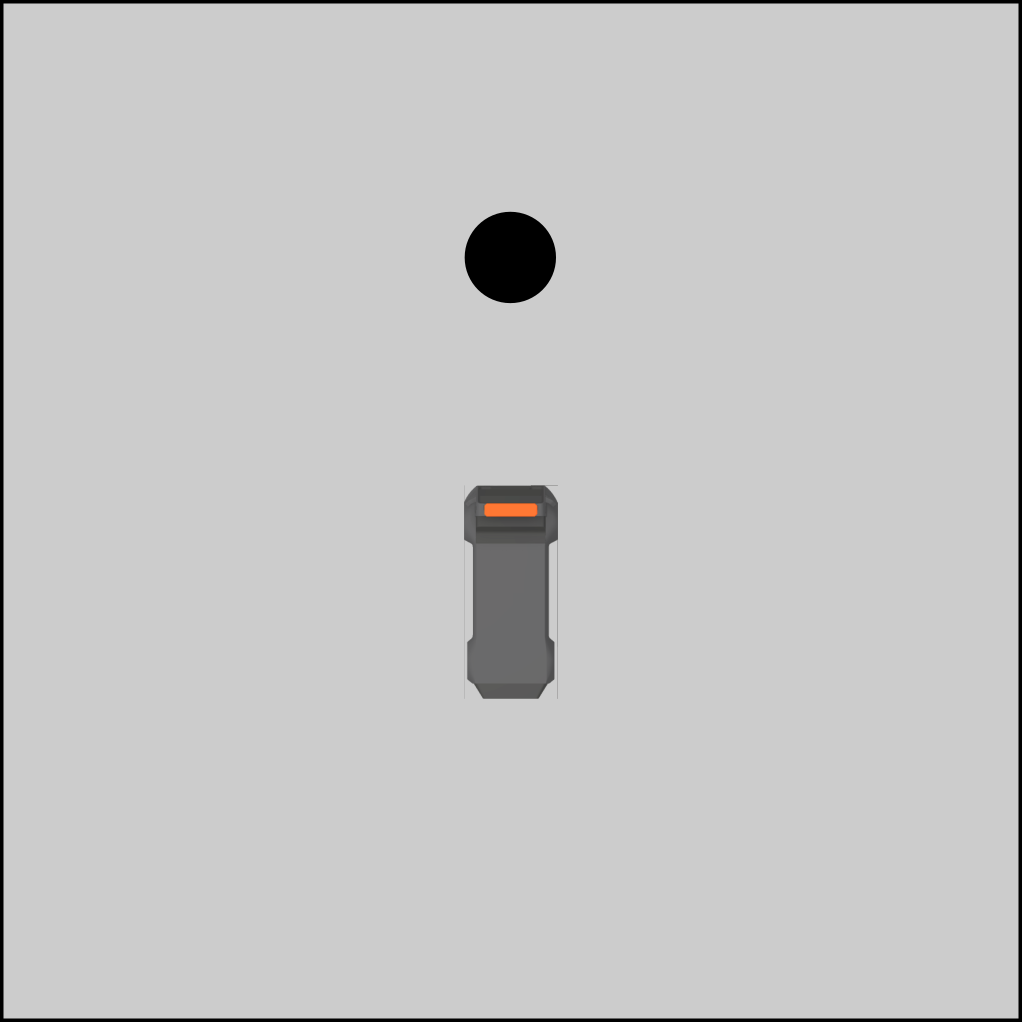
\includegraphics[width=0.3\linewidth]{images/bad_metrics_gt.png}}
		\hfill
		\subcaptionbox{Регистрация препятствия дальше эталонного положения.\label{fig:bad_metrics_far}}{%
			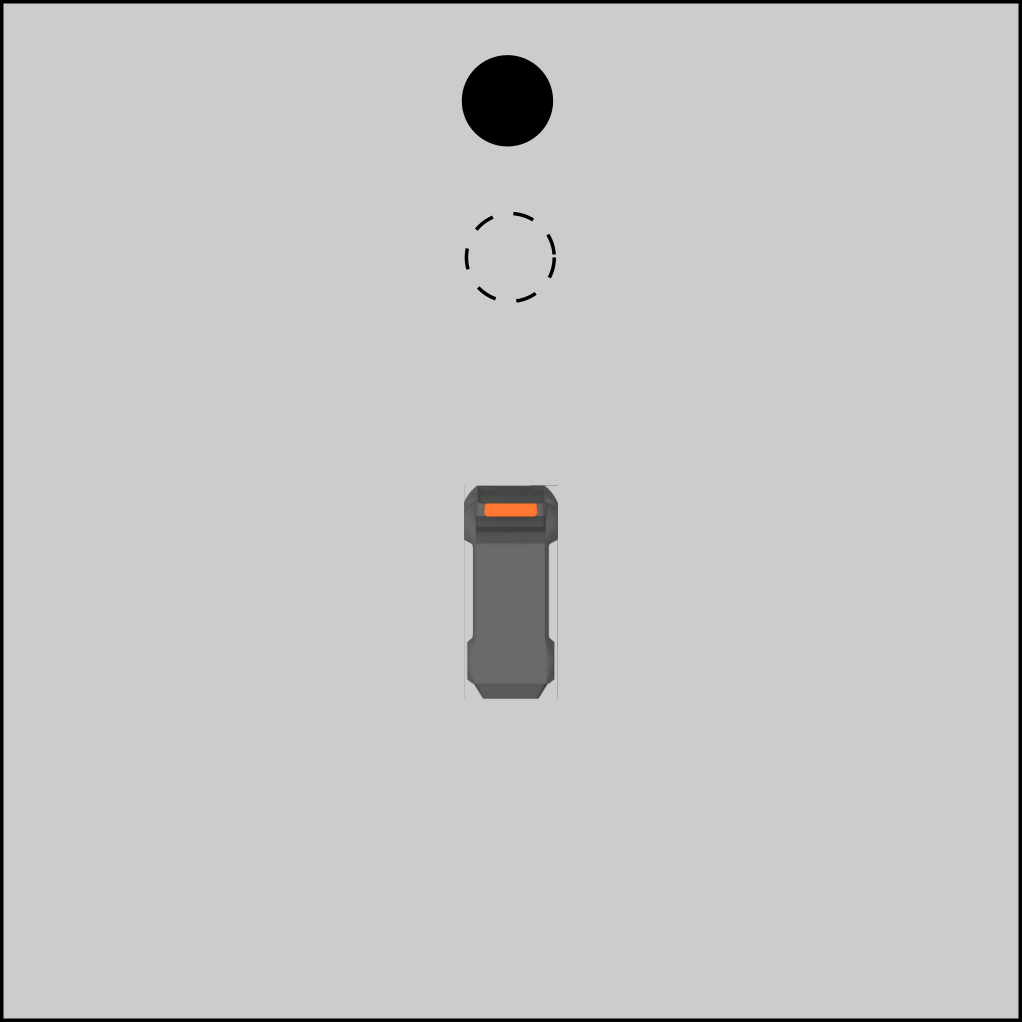
\includegraphics[width=0.3\linewidth]{images/bad_metrics_far.png}}
		\hfill
		\subcaptionbox{Регистрация препятствия ближе эталонного положения.\label{fig:bad_metrics_close}}{%
			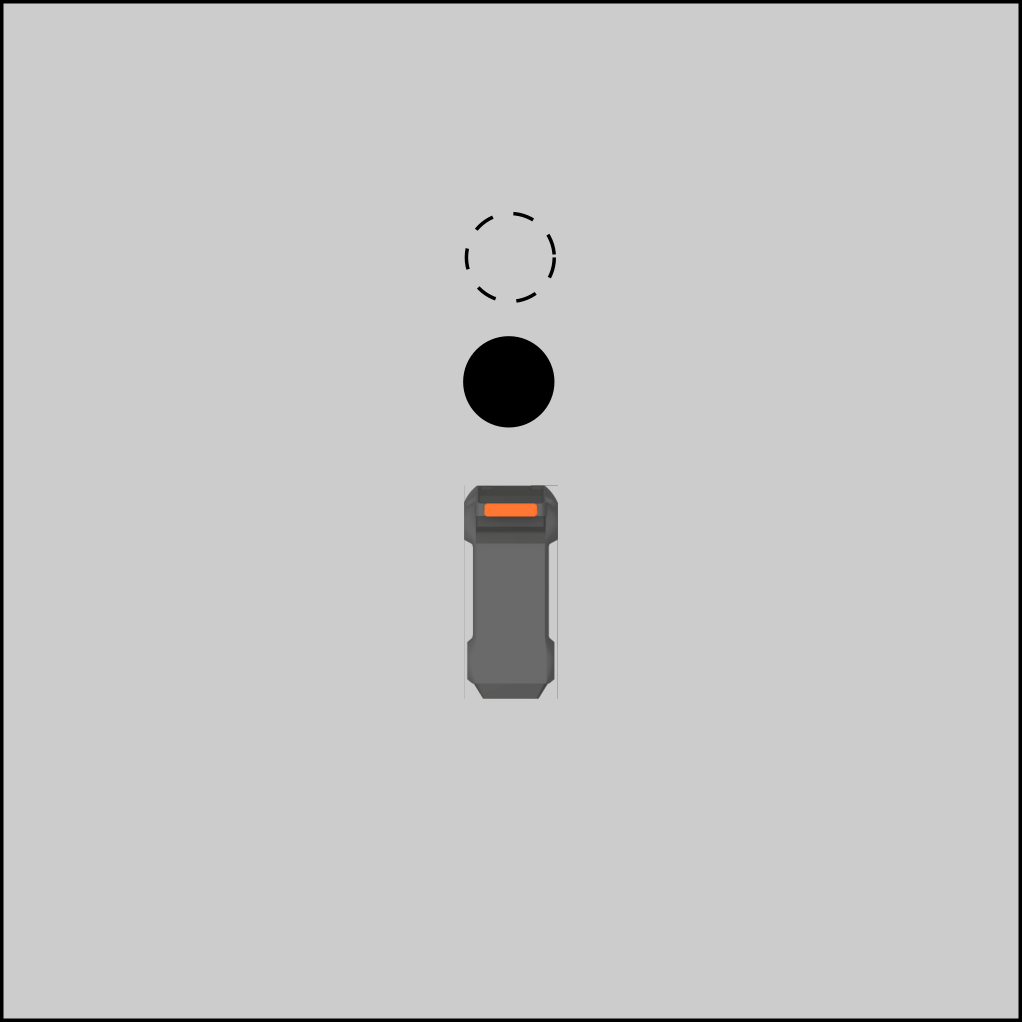
\includegraphics[width=0.3\linewidth]{images/bad_metrics_close.png}}
		\hfill
	}
	\caption{Пример эталонной карты и предсказанных карт с одинаковым качеством согласно метрикам, не учитывающим контекст решаемой задачи.}\label{fig:bad_metrics}
\end{figure}

Чтобы учесть это, в работе~\cite{horel2023navigation} была предложена метрика PathFinding Cost Mean Squared Error (PFC-MSE). Для её подсчёта производятся следующие шаги:

\begin{enumerate}
	\item Для каждого типа клетки выбирается стоимость её <<проезда>> $c>0$. Для клеток, соответствующих занятым областям, эта стоимость должна быть значительно выше, чем для свободных клеток (в оригинальной работе стоимость занятых клеток составила $cost_{occ} = 100$, свободных: $cost_{free} = 1$).
	\item Для эталонной и оцениваемой карт проходимости строятся ориентированные графы. Вершинами графа являются клетки карты, рёбрами соединены соседние клетки карты, вес ребра -- стоимость проезда клетки -- конечной вершины ребра, умноженная на расстояние между центрами клеток $w(c_1\rightarrow c_2) = cost(c_2) \cdot ||c_2 - c_1||_2$ (в оригинальной работе клетки, расположенные по диагонали, также считаются соседними).
	\item Используя алгоритм Дейкстры~\cite{cormen2009}, определяются пути с наименьшим весом $path\_cost(c)$ от центральной клетки карты, соответствующей положению БТС на карте.
	\item Для каждой клетки вес пути затем нормализуется: 
	
	$$path\_cost_{final}(c) = \dfrac{path\_cost(c) - L(c) \text{cost}_{free}}{\text{cost}_{occ} - \text{cost}_{free}},$$
	
	где $L(c)$ -- длина пути до вершины $c$. 
	\item Для построенных таким образом двух изображений (для эталонной и оцениваемой карт) находится среднеквадратичная ошибка, взвешенная вероятностью того, что соответствующая клетка является свободным пространством:
	
	$$\text{PFC-MSE}(GT, I) = \dfrac{\sum_c w_c||GT_{cost}(c) - I_{cost}(c)||_2}{\sum_c w_c},$$
	
	где $GT_{cost}$-- построенная карта нормализованных весов путей для эталонной карты, $I_{cost}$ -- для оцениваемой карты, $w_c = p(c = free)$.
\end{enumerate}

\subsection{Метрики для оценки непрерывных представлений}

Работы, представляющие модели из категории непрерывных представлений часто сравниваются с моделями сеточных представлений~\cite{Li2024, o2011continuous, 7487235}. Поэтому типичный подход к их оценке следующий: разбить пространство на сетку (двумерную или трёхмерную в зависимости от размерности оцениваемой модели), вычислить преобладающее значение внутри ограниченного клеткой пространства и тем самым преобразовать оцениваемую модель в модель сеточного представления, которую можно сравнивать с аналогами из этой категории. 

Для моделей, которые сопоставляют каждой точке пространства плотность вероятности нахождения в ней препятствия, стандартный подход к оценке качества -- построение рабочей характеристики приёмника (англ. Receiver operating characteristic, ROC). Каждой клетке после дискретизации пространства соответствует вероятность занятости соответствующего пространства, для вычисления ROC перебираются все возможные значения порога $p$, по которому бинаризуются значения клеток. Для полученной бинаризации вычисляется точность и полнота:

\begin{align*}
	Accuracy_p &= \dfrac{|TP_p|}{|TP_p| + |FP_p|}\\
	Recall_p &= \dfrac{|TP_p|}{|TP_p| + |FN_p|}.
\end{align*}

Полученное множество точек $(Accuracy_p, Recall_p)\in\left[0;1\right]^2$ образует ROC-кривую, площадь под которой (англ. Area Under Curve, AUC) описывает качество построенной модели.

\subsection{Выбор метрик для оценки предлагаемых алгоритмов}

Из рассмотренных метрик в настоящей работе используются следующие. Качество алгоритмов оценки положения объектов в окружающем пространстве БТС (глава~\cref{ch:ch2}) оценивается коэффициентом Жаккара $J$ и его усреднённым по объектам значением $mJ$: они непосредственно измеряют совпадение вычисленной и эталонной ограничивающих рамок и, в отличие от F-score и LocA, не требуют выбора порога $j_{thr}$, значение которого влияло бы на результат сравнения алгоритмов. Качество карты проходимости пространства, построенной с учётом визуальных данных, оценивается среднеквадратичной ошибкой относительно эталонной карты~\cref{eq:map_mse} и метрикой PFC-MSE: первая характеризует поклеточное расхождение моделей, вторая -- влияние этого расхождения на решение задачи планирования пути, ради которой модель и строится. Метрики отслеживания объектов и метрики непрерывных представлений в работе не используются, поскольку соответствующие задачи в ней не решаются.

\section{Требования к разрабатываемым алгоритмам и постановка задачи исследования}\label{sec:ch1/problem}

Проведённый обзор позволяет зафиксировать выбор базовой модели окружающего пространства, сформулировать требования к алгоритмам её построения и определить вытекающие из них подзадачи.

В качестве базовой модели в работе принята карта проходимости пространства (раздел~\cref{sec:ch1/sec2}). Выбор обоснован тремя обстоятельствами. Во-первых, модель описывает объекты произвольной геометрии и не требует их отнесения к заранее определённым классам, что существенно для БТС, движущегося в неструктурированной среде, где встречаются объекты, не представленные в обучающих выборках детекторов. Во-вторых, она допускает явное представление областей, о проходимости которых информация отсутствует, что необходимо для безопасного планирования пути в условиях окклюзии. В-третьих, принятый способ её обновления -- байесовский вывод с использованием обратной модели наблюдения (формула~\cref{eq:log_odd_upd}) -- сводит учёт данных отдельного источника к сложению независимо вычисленных слагаемых, что принципиально допускает одновременное обновление модели несколькими источниками данных.

Из результатов разделов~\cref{sec:ch1/sec3}--\cref{sec:ch1/performance} следуют требования к разрабатываемым алгоритмам:

\begin{enumerate}
	\item алгоритмы должны обеспечивать комплексирование данных камер и лидаров, поскольку ни один из этих типов датчиков в отдельности не позволяет одновременно получить высокое разрешение и непосредственное измерение расстояния (раздел~\cref{sec:ch1/sec3});
	\item алгоритмы проецирования данных камеры на плоскость движения БТС не должны опираться на предположение о совпадении поверхности движения с плоскостью, так как это предположение нарушается как рельефом местности, так и нормативными требованиями к профилю дорожного покрытия (раздел~\cref{sec:ch1/projection});
	\item алгоритмы должны выполняться в режиме реального времени на бортовом вычислителе БТС при ограниченных вычислительных ресурсах, что исключает применение методов, требующих инференса крупных нейросетевых моделей для каждого источника данных (разделы~\cref{sec:ch1/projection},~\cref{sec:ch1/performance});
	\item модель должна допускать подключение произвольного числа источников данных, в том числе новых, без изменения кода алгоритма построения карты;
	\item время внесения данных в модель не должно расти пропорционально числу источников данных, так как в противном случае число учитываемых датчиков оказывается ограничено сверху уже при скоростях движения, характерных для дорог общего пользования (раздел~\cref{sec:ch1/performance}, таблица~\cref{tab:sensors_limit}).
\end{enumerate}

Перечисленным требованиям соответствуют следующие подзадачи, решаемые в последующих главах работы:

\begin{enumerate}
	\item разработка алгоритмов проецирования визуальных детекций и семантической сегментации проезжей части с изображения на плоскость движения БТС на основе комплексирования данных камеры и лидара -- требования 1--3 (глава~\cref{ch:ch2});
	\item разработка программного комплекса, приводящего данные разнородных источников к единому представлению и осуществляющего их комплексирование в единой карте проходимости пространства, -- требование 4 (глава~\cref{ch:ch3});
	\item разработка алгоритма построения карты проходимости пространства, допускающего её одновременное обновление несколькими источниками данных, -- требование 5 (глава~\cref{ch:ch4}).
\end{enumerate}

\section{Заключение к главе \ref{ch:ch1}}\label{sec:ch1/sec6}

Итак, в рамках данной главы было выполнено следующее:

\begin{enumerate}
	\item проведён обзор существующих моделей представления окружающего пространства вокруг БТС. На основании проведённого обзора модель карты проходимости пространства была выбрана в качестве модели, которая будет использована для решения поставленных в работе задач;
	\item определены типичные виды датчиков, используемых на БТС для построения и уточнения моделей окружения, выделены преимущества и ограничения каждого из них. Сделан вывод о необходимости комплексирования данных с датчиков для построения более полной и точной модели окружения;
	\item проведён обзор существующих методов комплексирования данных;
	\item проведён обзор алгоритмов проецирования данных камеры на плоскость движения БТС. Показано, что существующие алгоритмы либо опираются на предположение о плоской поверхности движения, либо требуют вычислительных ресурсов, недоступных на бортовом вычислителе при одновременной обработке данных нескольких датчиков;
	\item рассмотрены вычислительные аспекты построения карты проходимости пространства при увеличении числа источников данных. Показано, что в существующих реализациях внесение данных в карту выполняется последовательно, и получена количественная оценка предельного числа источников данных, которые могут быть учтены в модели без потери её актуальности;
	\item определены основные метрики, используемые для оценки качества различных моделей представления окружающего пространства, и обоснован выбор метрик, применяемых в настоящей работе;
	\item сформулированы требования к разрабатываемым алгоритмам и определены подзадачи, решаемые в последующих главах работы.
\end{enumerate}

Решению первой из сформулированных подзадач -- разработке алгоритмов проецирования данных камеры на плоскость движения БТС -- посвящена следующая глава.

\begin{comment}
	
	
\section{Форматирование текста}\label{sec:ch1/sec1

Мы можем сделать \textbf{жирный текст} и \textit{курсив}.

\section{Ссылки}\label{sec:ch1/sec2}

Сошлёмся на библиографию.
Одна ссылка: \cite[с.~54]{Sokolov}\cite[с.~36]{Gaidaenko}.
Две ссылки: \cite{Sokolov,Gaidaenko}.
Ссылка на собственные работы: \cite{vakbib1, confbib2}.
Много ссылок: %\cite[с.~54]{Lermontov,Management,Borozda} % такой «фокус»
%вызывает biblatex warning относительно опции sortcites, потому что неясно, к
%какому источнику относится уточнение о страницах, а bibtex об этой проблеме
%даже не предупреждает
\cite{Lermontov, Management, Borozda, Marketing, Constitution, FamilyCode,
    Gost.7.0.53, Razumovski, Lagkueva, Pokrovski, Methodology, Berestova,
    Kriger}%
\ifnumequal{\value{bibliosel}}{0}{% Примеры для bibtex8
    \cite{Sirotko, Lukina, Encyclopedia, Nasirova}%
}{% Примеры для biblatex через движок biber
    \cite{Sirotko2, Lukina2, Encyclopedia2, Nasirova2}%
}%
.
И~ещё немного ссылок:~\cite{Article,Book,Booklet,Conference,Inbook,Incollection,Manual,Mastersthesis,
    Misc,Phdthesis,Proceedings,Techreport,Unpublished}
% Следует обратить внимание, что пробел после запятой внутри \cite{}
% обрабатывается ожидаемо, а пробел перед запятой, может вызывать проблемы при
% обработке ссылок.
\cite{medvedev2006jelektronnye, CEAT:CEAT581, doi:10.1080/01932691.2010.513279,
    Gosele1999161,Li2007StressAnalysis, Shoji199895, test:eisner-sample,
    test:eisner-sample-shorted, AB_patent_Pomerantz_1968, iofis_patent1960}%
\ifnumequal{\value{bibliosel}}{0}{% Примеры для bibtex8
}{% Примеры для biblatex через движок biber
    \cite{patent2h, patent3h, patent2}%
}%
.

\ifnumequal{\value{bibliosel}}{0}{% Примеры для bibtex8
Попытка реализовать несколько ссылок на конкретные страницы
для \texttt{bibtex} реализации библиографии:
[\citenum{Sokolov}, с.~54; \citenum{Gaidaenko}, с.~36].
}{% Примеры для biblatex через движок biber
Несколько источников (мультицитата):
% Тут специально написано по-разному тире, для демонстрации, что
% применение специальных тире в настоящий момент в biblatex приводит к непоказу
% "с.".
\cites[vii--x, 5, 7]{Sokolov}[v"--~x, 25, 526]{Gaidaenko}[vii--x, 5, 7]{Techreport},
работает только в \texttt{biblatex} реализации библиографии.
}%

Ссылки на собственные работы:~\cite{vakbib1, confbib1}.

Сошлёмся на приложения: Приложение~\cref{app:A}, Приложение~\cref{app:B2}.

Сошлёмся на формулу: формула~\cref{eq:equation1}.

Сошлёмся на изображение: рисунок~\cref{fig:knuth}.

Стандартной практикой является добавление к ссылкам префикса, характеризующего тип элемента.
Это не является строгим требованием, но~позволяет лучше ориентироваться в документах большого размера.
Например, для ссылок на~рисунки используется префикс \textit{fig},
для ссылки на~таблицу "--- \textit{tab}.

В таблице \cref{tab:tab_pref} приложения~\cref{app:B4} приведён список рекомендуемых
к использованию стандартных префиксов.

В некоторых ситуациях возникает необходимость отойти от требований ГОСТ по оформлению ссылок на
литературу.
В таком случае можно воспользоваться дополнительными опциями пакета \verb+biblatex+.

Например, в ссылке на книгу~\cite{sobenin_kdv} использование опции \verb+maxnames=4+ позволяет
вывести имена всех четырёх авторов.
По ГОСТ имена последних трёх авторов опускаются.

Кроме того, часто возникают проблемы с транслитерованными инициалами. Некоторые буквы русского
алфавита по правилам транслитерации записываются двумя буквами латинского алфавита (ю-yu, ё-yo и
т.д.).
Такие инициалы \verb+biblatex+ будет сокращать до одной буквы, что неверно.
Поправить его работу можно использовав опцию \verb+giveninits=false+.
Пример использования этой опции можно видеть в ссылке~\cite{initials}.

\section{Формулы}\label{sec:ch1/sec3}

Благодаря пакету \textit{icomma}, \LaTeX~одинаково хорошо воспринимает
в~качестве десятичного разделителя и запятую (\(3,1415\)), и точку (\(3.1415\)).

\subsection{Ненумерованные одиночные формулы}\label{subsec:ch1/sec3/sub1}

Вот так может выглядеть формула, которую необходимо вставить в~строку
по~тексту: \(x \approx \sin x\) при \(x \to 0\).

А вот так выглядит ненумерованная отдельностоящая формула c подстрочными
и надстрочными индексами:
\[
    (x_1+x_2)^2 = x_1^2 + 2 x_1 x_2 + x_2^2
\]

Формула с неопределенным интегралом:
\[
    \int f(\alpha+x)=\sum\beta
\]

При использовании дробей формулы могут получаться очень высокие:
\[
    \frac{1}{\sqrt{2}+
        \displaystyle\frac{1}{\sqrt{2}+
            \displaystyle\frac{1}{\sqrt{2}+\cdots}}}
\]

В формулах можно использовать греческие буквы:
%Все \original... команды заранее, ради этого примера, определены в Dissertation\userstyles.tex
\[
    \alpha\beta\gamma\delta\originalepsilon\epsilon\zeta\eta\theta%
    \vartheta\iota\kappa\varkappa\lambda\mu\nu\xi\pi\varpi\rho\varrho%
    \sigma\varsigma\tau\upsilon\originalphi\phi\chi\psi\omega\Gamma\Delta%
    \Theta\Lambda\Xi\Pi\Sigma\Upsilon\Phi\Psi\Omega
\]
\[%https://texfaq.org/FAQ-boldgreek
    \boldsymbol{\alpha\beta\gamma\delta\originalepsilon\epsilon\zeta\eta%
        \theta\vartheta\iota\kappa\varkappa\lambda\mu\nu\xi\pi\varpi\rho%
        \varrho\sigma\varsigma\tau\upsilon\originalphi\phi\chi\psi\omega\Gamma%
        \Delta\Theta\Lambda\Xi\Pi\Sigma\Upsilon\Phi\Psi\Omega}
\]

Для добавления формул можно использовать пары \verb+$+\dots\verb+$+ и \verb+$$+\dots\verb+$$+,
но~они считаются устаревшими.
Лучше использовать их функциональные аналоги \verb+\(+\dots\verb+\)+ и \verb+\[+\dots\verb+\]+.

\subsection{Ненумерованные многострочные формулы}\label{subsec:ch1/sec3/sub2}

Вот так можно написать две формулы, не нумеруя их, чтобы знаки <<равно>> были
строго друг под другом:
\begin{align}
    f_W & =  \min \left( 1, \max \left( 0, \frac{W_{soil} / W_{max}}{W_{crit}} \right)  \right), \nonumber \\
    f_T & =  \min \left( 1, \max \left( 0, \frac{T_s / T_{melt}}{T_{crit}} \right)  \right), \nonumber
\end{align}

Выровнять систему ещё и по переменной \( x \) можно, используя окружение
\verb|alignedat| из пакета \verb|amsmath|. Вот так:
\[
|x| = \left\{
\begin{alignedat}{2}
     &   & x, \quad & \text{eсли } x\geqslant 0 \\
     & - & x, \quad & \text{eсли } x<0
\end{alignedat}
\right.
\]
Здесь первый амперсанд (в исходном \LaTeX\ описании формулы) означает
выравнивание по~левому краю, второй "--- по~\( x \), а~третий "--- по~слову
<<если>>. Команда \verb|\quad| делает большой горизонтальный пробел.

Ещё вариант:
\[
    |x|=
    \begin{cases}
        \phantom{-}x, \text{если } x \geqslant 0 \\
        -x, \text{если } x<0
    \end{cases}
\]

Кроме того, для  нумерованных формул \verb|alignedat| делает вертикальное
выравнивание номера формулы по центру формулы. Например, выравнивание
компонент вектора:
\begin{equation}
    \label{eq:2p3}
    \begin{alignedat}{2}
        {\mathbf{N}}_{o1n}^{(j)} = \,{\sin} \phi\,n\!\left(n+1\right)
        {\sin}\theta\,
        \pi_n\!\left({\cos} \theta\right)
        \frac{
        z_n^{(j)}\!\left( \rho \right)
        }{\rho}\,
         & {\boldsymbol{\hat{\mathrm e}}}_{r}\,+      \\
        +\,
        {\sin} \phi\,
        \tau_n\!\left({\cos} \theta\right)
        \frac{
        \left[\rho z_n^{(j)}\!\left( \rho \right)\right]^{\prime}
        }{\rho}\,
         & {\boldsymbol{\hat{\mathrm e}}}_{\theta}\,+ \\
        +\,
        {\cos} \phi\,
        \pi_n\!\left({\cos} \theta\right)
        \frac{
        \left[\rho z_n^{(j)}\!\left( \rho \right)\right]^{\prime}
        }{\rho}\,
         & {\boldsymbol{\hat{\mathrm e}}}_{\phi}\:.
    \end{alignedat}
\end{equation}

Ещё об отступах. Иногда для лучшей <<читаемости>> формул полезно
немного исправить стандартные интервалы \LaTeX\ с учётом логической
структуры самой формулы. Например в формуле~\cref{eq:2p3} добавлен
небольшой отступ \verb+\,+ между основными сомножителями, ниже
результат применения всех вариантов отступа:
\begin{align*}
    \backslash!             & \quad f(x) = x^2\! +3x\! +2         \\
    \mbox{по-умолчанию}     & \quad f(x) = x^2+3x+2               \\
    \backslash,             & \quad f(x) = x^2\, +3x\, +2         \\
    \backslash{:}           & \quad f(x) = x^2\: +3x\: +2         \\
    \backslash;             & \quad f(x) = x^2\; +3x\; +2         \\
    \backslash \mbox{space} & \quad f(x) = x^2\ +3x\ +2           \\
    \backslash \mbox{quad}  & \quad f(x) = x^2\quad +3x\quad +2   \\
    \backslash \mbox{qquad} & \quad f(x) = x^2\qquad +3x\qquad +2
\end{align*}

Можно использовать разные математические алфавиты:
\begin{align}
    \mathcal{ABCDEFGHIJKLMNOPQRSTUVWXYZ} \nonumber  \\
    \mathfrak{ABCDEFGHIJKLMNOPQRSTUVWXYZ} \nonumber \\
    \mathbb{ABCDEFGHIJKLMNOPQRSTUVWXYZ} \nonumber
\end{align}

Посмотрим на систему уравнений на примере аттрактора Лоренца:

\[
\left\{
\begin{array}{rl}
    \dot x = & \sigma (y-x)  \\
    \dot y = & x (r - z) - y \\
    \dot z = & xy - bz
\end{array}
\right.
\]

А для вёрстки матриц удобно использовать многоточия:
\[
    \left(
        \begin{array}{ccc}
            a_{11} & \ldots & a_{1n} \\
            \vdots & \ddots & \vdots \\
            a_{n1} & \ldots & a_{nn} \\
        \end{array}
    \right)
\]

\subsection{Нумерованные формулы}\label{subsec:ch1/sec3/sub3}

А вот так пишется нумерованная формула:
\begin{equation}
    \label{eq:equation1}
    e = \lim_{n \to \infty} \left( 1+\frac{1}{n} \right) ^n
\end{equation}

Нумерованных формул может быть несколько:
\begin{equation}
    \label{eq:equation2}
    \lim_{n \to \infty} \sum_{k=1}^n \frac{1}{k^2} = \frac{\pi^2}{6}
\end{equation}

Впоследствии на формулы~\cref{eq:equation1, eq:equation2} можно ссылаться.

Сделать так, чтобы номер формулы стоял напротив средней строки, можно,
используя окружение \verb|multlined| (пакет \verb|mathtools|) вместо
\verb|multline| внутри окружения \verb|equation|. Вот так:
\begin{equation} % \tag{S} % tag - вписывает свой текст
    \label{eq:equation3}
    \begin{multlined}
        1+ 2+3+4+5+6+7+\dots + \\
        + 50+51+52+53+54+55+56+57 + \dots + \\
        + 96+97+98+99+100=5050
    \end{multlined}
\end{equation}

Уравнения~\cref{eq:subeq_1,eq:subeq_2} демонстрируют возможности
окружения \verb|subequations| (пакет \verb|amsmath|).
\begin{subequations}
    \label{eq:subeq_1}
    \begin{gather}
        y = x^2 + 1 \label{eq:subeq_1-1} \\
        y = 2 x^2 - x + 1 \label{eq:subeq_1-2}
    \end{gather}
\end{subequations}
Ссылки на отдельные уравнения~\cref{eq:subeq_1-1,eq:subeq_1-2,eq:subeq_2-1}.
\begin{subequations}
    \label{eq:subeq_2}
    \begin{align}
        y & = x^3 + x^2 + x + 1 \label{eq:subeq_2-1} \\
        y & = x^2
    \end{align}
\end{subequations}

\subsection{Форматирование чисел и размерностей величин}\label{sec:units}

Числа форматируются при помощи команды \verb|\num|:
\num{5,3};
\num{2,3e8};
\num{12345,67890};
\num{2,6 d4};
\num{1+-2i};
\num{.3e45};
\num[exponent-base=2]{5 e64};
\num[exponent-base=2,exponent-to-prefix]{5 e64};
\num{1.654 x 2.34 x 3.430}
\num{1 2 x 3 / 4}.
Для написания последовательности чисел можно использовать команды \verb|\numlist| и \verb|\numrange|:
\numlist{10;30;50;70}; \numrange{10}{30}.
Значения углов можно форматировать при помощи команды \verb|\ang|:
\ang{2.67};
\ang{30,3};
\ang{-1;;};
\ang{;-2;};
\ang{;;-3};
\ang{300;10;1}.

Обратите внимание, что ГОСТ запрещает использование знака <<->> для обозначения отрицательных чисел
за исключением формул, таблиц и~рисунков.
Вместо него следует использовать слово <<минус>>.

Размерности можно записывать при помощи команд \verb|\si| и \verb|\SI|:
\si{\farad\squared\lumen\candela};
\si{\joule\per\mole\per\kelvin};
\si[per-mode = symbol-or-fraction]{\joule\per\mole\per\kelvin};
\si{\metre\per\second\squared};
\SI{0.10(5)}{\neper};
\SI{1.2-3i e5}{\joule\per\mole\per\kelvin};
\SIlist{1;2;3;4}{\tesla};
\SIrange{50}{100}{\volt}.
Список единиц измерений приведён в таблицах~\cref{tab:unit:base,
    tab:unit:derived,tab:unit:accepted,tab:unit:physical,tab:unit:other}.
Приставки единиц приведены в~таблице~\cref{tab:unit:prefix}.

С дополнительными опциями форматирования можно ознакомиться в~описании пакета \texttt{siunitx};
изменить или добавить единицы измерений можно в~файле \texttt{siunitx.cfg}.

\begin{table}
    \centering
    \captionsetup{justification=centering} % выравнивание подписи по-центру
    \caption{Основные величины СИ}\label{tab:unit:base}
    \begin{tabular}{llc}
        \toprule
        Название  & Команда          & Символ         \\
        \midrule
        Ампер     & \verb|\ampere|   & \si{\ampere}   \\
        Кандела   & \verb|\candela|  & \si{\candela}  \\
        Кельвин   & \verb|\kelvin|   & \si{\kelvin}   \\
        Килограмм & \verb|\kilogram| & \si{\kilogram} \\
        Метр      & \verb|\metre|    & \si{\metre}    \\
        Моль      & \verb|\mole|     & \si{\mole}     \\
        Секунда   & \verb|\second|   & \si{\second}   \\
        \bottomrule
    \end{tabular}
\end{table}

\begin{table}
    \small
    \centering
    \begin{threeparttable}% выравнивание подписи по границам таблицы
        \caption{Производные единицы СИ}\label{tab:unit:derived}
        \begin{tabular}{llc|llc}
            \toprule
            Название       & Команда               & Символ              & Название & Команда & Символ \\
            \midrule
            Беккерель      & \verb|\becquerel|     & \si{\becquerel}     &
            Ньютон         & \verb|\newton|        & \si{\newton}                                      \\
            Градус Цельсия & \verb|\degreeCelsius| & \si{\degreeCelsius} &
            Ом             & \verb|\ohm|           & \si{\ohm}                                         \\
            Кулон          & \verb|\coulomb|       & \si{\coulomb}       &
            Паскаль        & \verb|\pascal|        & \si{\pascal}                                      \\
            Фарад          & \verb|\farad|         & \si{\farad}         &
            Радиан         & \verb|\radian|        & \si{\radian}                                      \\
            Грей           & \verb|\gray|          & \si{\gray}          &
            Сименс         & \verb|\siemens|       & \si{\siemens}                                     \\
            Герц           & \verb|\hertz|         & \si{\hertz}         &
            Зиверт         & \verb|\sievert|       & \si{\sievert}                                     \\
            Генри          & \verb|\henry|         & \si{\henry}         &
            Стерадиан      & \verb|\steradian|     & \si{\steradian}                                   \\
            Джоуль         & \verb|\joule|         & \si{\joule}         &
            Тесла          & \verb|\tesla|         & \si{\tesla}                                       \\
            Катал          & \verb|\katal|         & \si{\katal}         &
            Вольт          & \verb|\volt|          & \si{\volt}                                        \\
            Люмен          & \verb|\lumen|         & \si{\lumen}         &
            Ватт           & \verb|\watt|          & \si{\watt}                                        \\
            Люкс           & \verb|\lux|           & \si{\lux}           &
            Вебер          & \verb|\weber|         & \si{\weber}                                       \\
            \bottomrule
        \end{tabular}
    \end{threeparttable}
\end{table}

\begin{table}
    \centering
    \begin{threeparttable}% выравнивание подписи по границам таблицы
        \caption{Внесистемные единицы}\label{tab:unit:accepted}

        \begin{tabular}{llc}
            \toprule
            Название        & Команда           & Символ          \\
            \midrule
            День            & \verb|\day|       & \si{\day}       \\
            Градус          & \verb|\degree|    & \si{\degree}    \\
            Гектар          & \verb|\hectare|   & \si{\hectare}   \\
            Час             & \verb|\hour|      & \si{\hour}      \\
            Литр            & \verb|\litre|     & \si{\litre}     \\
            Угловая минута  & \verb|\arcminute| & \si{\arcminute} \\
            Угловая секунда & \verb|\arcsecond| & \si{\arcsecond} \\ %
            Минута          & \verb|\minute|    & \si{\minute}    \\
            Тонна           & \verb|\tonne|     & \si{\tonne}     \\
            \bottomrule
        \end{tabular}
    \end{threeparttable}
\end{table}

\begin{table}
    \centering
    \captionsetup{justification=centering}
    \caption{Внесистемные единицы, получаемые из эксперимента}\label{tab:unit:physical}
    \begin{tabular}{llc}
        \toprule
        Название                & Команда                  & Символ                 \\
        \midrule
        Астрономическая единица & \verb|\astronomicalunit| & \si{\astronomicalunit} \\
        Атомная единица массы   & \verb|\atomicmassunit|   & \si{\atomicmassunit}   \\
        Боровский радиус        & \verb|\bohr|             & \si{\bohr}             \\
        Скорость света          & \verb|\clight|           & \si{\clight}           \\
        Дальтон                 & \verb|\dalton|           & \si{\dalton}           \\
        Масса электрона         & \verb|\electronmass|     & \si{\electronmass}     \\
        Электрон Вольт          & \verb|\electronvolt|     & \si{\electronvolt}     \\
        Элементарный заряд      & \verb|\elementarycharge| & \si{\elementarycharge} \\
        Энергия Хартри          & \verb|\hartree|          & \si{\hartree}          \\
        Постоянная Планка       & \verb|\planckbar|        & \si{\planckbar}        \\
        \bottomrule
    \end{tabular}
\end{table}

\begin{table}
    \centering
    \begin{threeparttable}% выравнивание подписи по границам таблицы
        \caption{Другие внесистемные единицы}\label{tab:unit:other}
        \begin{tabular}{llc}
            \toprule
            Название                  & Команда              & Символ             \\
            \midrule
            Ангстрем                  & \verb|\angstrom|     & \si{\angstrom}     \\
            Бар                       & \verb|\bar|          & \si{\bar}          \\
            Барн                      & \verb|\barn|         & \si{\barn}         \\
            Бел                       & \verb|\bel|          & \si{\bel}          \\
            Децибел                   & \verb|\decibel|      & \si{\decibel}      \\
            Узел                      & \verb|\knot|         & \si{\knot}         \\
            Миллиметр ртутного столба & \verb|\mmHg|         & \si{\mmHg}         \\
            Морская миля              & \verb|\nauticalmile| & \si{\nauticalmile} \\
            Непер                     & \verb|\neper|        & \si{\neper}        \\
            \bottomrule
        \end{tabular}
    \end{threeparttable}
\end{table}

\begin{table}
    \small
    \centering
    \begin{threeparttable}% выравнивание подписи по границам таблицы
        \caption{Приставки СИ}\label{tab:unit:prefix}
        \begin{tabular}{llcc|llcc}
            \toprule
            Приставка & Команда       & Символ      & Степень      &
            Приставка & Команда       & Символ      & Степень        \\
            \midrule
            Иокто     & \verb|\yocto| & \si{\yocto} & \textminus24 &
            Дека      & \verb|\deca|  & \si{\deca}  & 1              \\
            Зепто     & \verb|\zepto| & \si{\zepto} & \textminus21 &
            Гекто     & \verb|\hecto| & \si{\hecto} & 2              \\
            Атто      & \verb|\atto|  & \si{\atto}  & \textminus18 &
            Кило      & \verb|\kilo|  & \si{\kilo}  & 3              \\
            Фемто     & \verb|\femto| & \si{\femto} & \textminus15 &
            Мега      & \verb|\mega|  & \si{\mega}  & 6              \\
            Пико      & \verb|\pico|  & \si{\pico}  & \textminus12 &
            Гига      & \verb|\giga|  & \si{\giga}  & 9              \\
            Нано      & \verb|\nano|  & \si{\nano}  & \textminus9  &
            Терра     & \verb|\tera|  & \si{\tera}  & 12             \\
            Микро     & \verb|\micro| & \si{\micro} & \textminus6  &
            Пета      & \verb|\peta|  & \si{\peta}  & 15             \\
            Милли     & \verb|\milli| & \si{\milli} & \textminus3  &
            Екса      & \verb|\exa|   & \si{\exa}   & 18             \\
            Санти     & \verb|\centi| & \si{\centi} & \textminus2  &
            Зетта     & \verb|\zetta| & \si{\zetta} & 21             \\
            Деци      & \verb|\deci|  & \si{\deci}  & \textminus1  &
            Иотта     & \verb|\yotta| & \si{\yotta} & 24             \\
            \bottomrule
        \end{tabular}
    \end{threeparttable}
\end{table}

\subsection{Заголовки с формулами: \texorpdfstring{\(a^2 + b^2 = c^2\)}{%
        a\texttwosuperior\ + b\texttwosuperior\ = c\texttwosuperior},
    \texorpdfstring{\(\left\vert\textrm{{Im}}\Sigma\left(
            \protect\varepsilon\right)\right\vert\approx const\)}{|ImΣ (ε)| ≈ const},
    \texorpdfstring{\(\sigma_{xx}^{(1)}\)}{σ\_\{xx\}\textasciicircum\{(1)\}}
}\label{subsec:with_math}

Пакет \texttt{hyperref} берёт текст для закладок в pdf-файле из~аргументов
команд типа \verb|\section|, которые могут содержать математические формулы,
а~также изменения цвета текста или шрифта, которые не отображаются в~закладках.
Чтобы использование формул в заголовках не вызывало в~логе компиляции появление
предупреждений типа <<\texttt{Token not allowed in~a~PDF string
    (Unicode):(hyperref) removing...}>>, следует использовать конструкцию
\verb|\texorpdfstring{}{}|, где в~первых фигурных скобках указывается
формула, а~во~вторых "--- запись формулы для закладок.

\section{Рецензирование текста}\label{sec:markup}

В шаблоне для диссертации и автореферата заданы команды рецензирования.
Они видны при компиляции шаблона в режиме черновика или при установке
соответствующей настройки (\verb+showmarkup+) в~файле \verb+common/setup.tex+.

Команда \verb+\todo+ отмечает текст красным цветом.
\todo{Например, так.}

Команда \verb+\note+ позволяет выбрать цвет текста.
\note{Чёрный, } \note[red]{красный, } \note[green]{зелёный, }
\note[blue]{синий.} \note[orange]{Обратите внимание на ширину и расстановку
    формирующихся пробелов, в~результате приведённой записи (зависит также
    от~применяемого компилятора).}

Окружение \verb+commentbox+ также позволяет выбрать цвет.

\begin{commentbox}[red]
    Красный текст.

    Несколько параграфов красного текста.
\end{commentbox}

\begin{commentbox}[blue]
    Синяя формула.

    \begin{equation}
        \alpha + \beta = \gamma
    \end{equation}
\end{commentbox}

\verb+commentbox+ позволяет закомментировать участок кода в~режиме чистовика.
Чтобы убрать кусок кода для всех режимов, можно использовать окружение
\verb+comment+.



\section{Работа со списком сокращений и~условных обозначений}\label{sec:acronyms}

С помощью пакета \texttt{nomencl} можно создавать удобный сортированный список
сокращений и условных обозначений во время написания текста. Вызов
\verb+\nomenclature+ добавляет нужный символ или сокращение с~описанием
в~список, который затем печатается вызовом \verb+\printnomenclature+
в~соответствующем разделе.
Для того, чтобы эти операции прошли, потребуется дополнительный вызов
\verb+makeindex -s nomencl.ist -o %.nls %.nlo+ в~командной строке, где вместо
\verb+%+ следует подставить имя главного файла проекта (\verb+dissertation+
для этого шаблона).
Затем потребуется один или два дополнительных вызова компилятора проекта.
\begin{equation}
    \omega = c k,
\end{equation}
где \( \omega \) "--- частота света, \( c \) "--- скорость света, \( k \) "---
модуль волнового вектора.
\nomenclature{\(\omega\)}{частота света\nomrefeq}
\nomenclature{\(c\)}{скорость света\nomrefpage}
\nomenclature{\(k\)}{модуль волнового вектора\nomrefeqpage}
Использование
\begin{verbatim}
\nomenclature{\(\omega\)}{частота света\nomrefeq}
\nomenclature{\(c\)}{скорость света\nomrefpage}
\nomenclature{\(k\)}{модуль волнового вектора\nomrefeqpage}
\end{verbatim}
после уравнения добавит в список условных обозначений три записи.
Ссылки \verb+\nomrefeq+ на последнее уравнение, \verb+\nomrefpage+ "--- на
страницу, \verb+\nomrefeqpage+ "--- сразу на~последнее уравнение и~на~страницу,
можно опускать и~не~использовать.

Группировкой и сортировкой пунктов в списке можно управлять с~помощью указания
дополнительных аргументов к команде \verb+nomenclature+.
Например, при вызове
\begin{verbatim}
\nomenclature[03]{\( \hbar \)}{постоянная Планка}
\nomenclature[01]{\( G \)}{гравитационная постоянная}
\end{verbatim}
\( G \) будет стоять в списке выше, чем \( \hbar \).
Для корректных вертикальных отступов между строками в описании лучше
не~использовать многострочные формулы в~списке обозначений.

\nomenclature{%
    \( \begin{rcases}
        a_n \\
        b_n
    \end{rcases} \)%
}{коэффициенты разложения Ми в дальнем поле соответствующие электрическим и
    магнитным мультиполям}
\nomenclature[a\( e \)]{\( {\boldsymbol{\hat{\mathrm e}}} \)}{единичный вектор}
\nomenclature{\( E_0 \)}{амплитуда падающего поля}
\nomenclature{\( j \)}{тип функции Бесселя}
\nomenclature{\( k \)}{волновой вектор падающей волны}
\nomenclature{%
    \( \begin{rcases}
        a_n \\
        b_n
    \end{rcases} \)%
}{и снова коэффициенты разложения Ми в дальнем поле соответствующие
    электрическим и магнитным мультиполям. Добавлено много текста, так что
    описание группы условных обозначений значительно превысило высоту этой
    группы...}
\nomenclature{\( L \)}{общее число слоёв}
\nomenclature{\( l \)}{номер слоя внутри стратифицированной сферы}
\nomenclature{\( \lambda \)}{длина волны электромагнитного излучения в вакууме}
\nomenclature{\( n \)}{порядок мультиполя}
\nomenclature{%
    \( \begin{rcases}
        {\mathbf{N}}_{e1n}^{(j)} & {\mathbf{N}}_{o1n}^{(j)} \\
        {\mathbf{M}_{o1n}^{(j)}} & {\mathbf{M}_{e1n}^{(j)}}
    \end{rcases} \)%
}{сферические векторные гармоники}
\nomenclature{\( \mu \)}{магнитная проницаемость в вакууме}
\nomenclature{\( r, \theta, \phi \)}{полярные координаты}
\nomenclature{\( \omega \)}{частота падающей волны}

С помощью \verb+nomenclature+ можно включать в~список сокращения,
не~используя их~в~тексте.
% запись сокращения в список происходит командой \nomenclature,
% а не употреблением самого сокращения
\nomenclature{FEM}{finite element method, метод конечных элементов}
\nomenclature{FIT}{finite integration technique, метод конечных интегралов}
\nomenclature{FMM}{fast multipole method, быстрый метод многополюсника}
\nomenclature{FVTD}{finite volume time-domain, метод конечных объёмов
    во~временной области}
\nomenclature{MLFMA}{multilevel fast multipole algorithm, многоуровневый
    быстрый алгоритм многополюсника}
\nomenclature{BEM}{boundary element method, метод граничных элементов}
\nomenclature{CST MWS}{Computer Simulation Technology Microwave Studio
    программа для компьютерного моделирования уравнен Максвелла}
\nomenclature{DDA}{discrete dipole approximation, приближение дискретиных
    диполей}
\nomenclature{FDFD}{finite difference frequency domain, метод конечных
    разностей в~частотной области}
\nomenclature{FDTD}{finite difference time domain, метод конечных разностей
    во~временной области}
\nomenclature{MoM}{method of moments, метод моментов}
\nomenclature{MSTM}{multiple sphere T-Matrix, метод Т-матриц для множества
    сфер}
\nomenclature{PSTD}{pseudospectral time domain method, псевдоспектральный метод
    во~временной области}
\nomenclature{TLM}{transmission line matrix method, метод матриц линий передач}
\end{comment}
\FloatBarrier
